\section{Comparative Analysis of Security Controls}\label{sec:controls}
\answers{Answers RQ2}

\paragraph*{Rubric} We score fifteen control dimensions from 0 to 3: D01 permission model, D02 execution sandbox, D03 network egress, D04 workspace and configuration trust, D05 MCP governance, D06 extensions and plugins, D07 secrets and credential storage, D08 headless and CI safeguards, D09 persistent memory, D10 sub-agent isolation, D11 audit logging, D12 telemetry and retention, D13 distribution supply chain, D14 managed policy and D15 vulnerability disclosure. The scale reads 0~absent, 1~opt-in or weak, 2~on by default with documented gaps, and 3~strong, documented and centrally enforceable, with per-dimension criteria (Appendix~\ref{app:rubric}). Only \evD{} and \evT{} facts can raise a score; \evTP{} facts can only lower one, since third-party reports document bypasses rather than guarantees. The score is the highest level whose criteria are \emph{all} met; an undecidable criterion counts as unmet; incident history, which belongs to RQ3, leaves scores unchanged. Means are unweighted, require at least eight scored dimensions and are reported alongside the minimum; a ranking is asserted only where it holds under equal, incident-exposure and security-core weightings alike.

\paragraph*{Coverage and reliability} Of \nCells{} harness--dimension cells, \nCellsScored{} were scored and \nCellsNA{} are N/A with a recorded reason (feature absent, no access, or undocumented); \nInsufficientEOne{} runtimes have too little evidence to support a mean. A second LLM-agent rater, blind to the first rater's scores, rescored the matrix from the \emph{same} extracted fact lists, so agreement measures how consistently the rubric is applied to shared evidence, not the reliability of evidence collection. On the \nOverlapEOne{} cells both raters scored, quadratic-weighted Cohen's $\kappa$~\cite{cohen1968} is \kappaEOne{}, exact agreement \exactEOne{} and within-one agreement \withinOneEOne{}; these figures exclude the \naVsScoreEOne{} cells in which one rater recorded N/A and the other a score. All \nDisagreeEOne{} disagreements, those N/A cases included, are published rather than adjudicated, and rater~1's scores are reported.

\begin{figure}[!t]
\centering
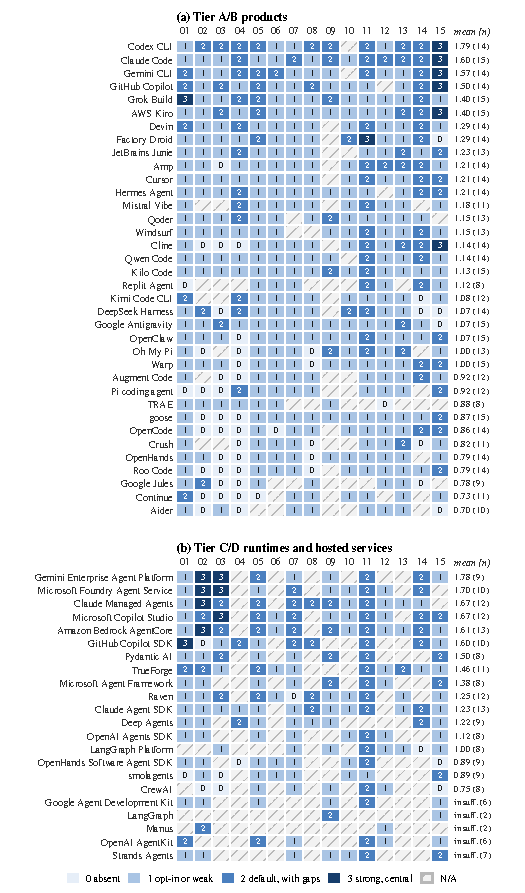
\includegraphics[width=0.9\columnwidth]{figures/e1_heatmap.pdf}
\caption{Control matrix (RQ2): score 0--3 per dimension, rater~1; hatched cells are N/A. Tier A/B products (top) and tier C/D runtimes and hosted services (bottom) are ranked separately. The same scores with means are generated as \texttt{paper/tables/scorecard.tex}; per-cell evidence and rationale are in \texttt{matrix/}.}
\label{fig:heatmap}
\end{figure}

\paragraph*{Overall picture} Controls exist but are seldom safe by default (Figure~\ref{fig:heatmap}). Across the \nRankedAB{} tier A/B products no per-dimension mean reaches 2. The lowest means belong to network egress (D03, \dimABMeanThree{}), the execution sandbox (D02, \dimABMeanTwo{}), headless and CI safeguards (D08, \dimABMeanEight{}) and workspace trust (D04, \dimABMeanFour{}); the highest to vulnerability disclosure (D15, \dimABMeanFifteen{}), audit logging (D11, \dimABMeanEleven{}) and managed policy (D14, \dimABMeanFourteen{}). Overall means are closely bunched: only Codex CLI stays in the top three, and only Continue in the bottom three, under every weighting, so the per-dimension columns are more informative than the means.

\paragraph*{Permission model (D01)} Nearly every product offers per-action approval, yet only \dimABTwoPlusOne{} of \nRankedAB{} reach score~2. Two patterns depress the scores: approve-everything can often be enabled from repository-controlled files, through hooks that return an auto-approve verdict or repository MCP entries carrying \texttt{autoApprove}; and several harnesses default to a model-based approver (Claude Code's \texttt{auto}\evD{}, Cursor's auto-review\evD{}, Qwen Code's AUTO\evD{}, Hermes Agent's \texttt{smart}\evD{}). The rubric does not treat a classifier's verdict as ``asking'', so these defaults score~1. Counting them as asking would raise Claude Code's D01 from 1 to 3 and lift the other classifier-default harnesses; we did not recompute the rankings under that reading, which remains the rubric's principal open question.

\paragraph*{Sandbox and egress (D02, D03)} These are the lowest-scoring dimensions (means \dimABMeanTwo{} and \dimABMeanThree{}). Among tier A/B products, \dimABZeroTwo{} offer no sandbox at all, \dimABThreeTwo{} confine both filesystem and network by default with central enforcement (score~3), and \dimABZeroThree{} have no egress control. Managed runtimes score higher (tier C/D means \dimCMeanTwo{} and \dimCMeanThree{}) because the provider runs each session in an isolated container or microVM. Where sandboxes exist, the incident record shows their boundaries to be a frequent point of failure: symlink and working-directory tricks, writes to \texttt{.git} hooks and fallbacks to unsandboxed execution account for \nIncTSeventeen{} escape incidents (Section~\ref{sec:incidents}).

\paragraph*{Workspace trust (D04)} Repository configuration is honoured with no notion of trust by \dimABZeroFour{} tier A/B products, and none reaches score~3. A recurrent design choice is that headless mode bypasses the trust gate. Claude Code documents that \texttt{claude -p} in a never-trusted folder runs project hooks and MCP servers\evD~\cite{cc_permissions_trust}, which we observed\evT{}; by contrast, Grok Build ran an untrusted repository hook only after \texttt{--trust}\evD\evT{}, and Copilot CLI did not start a repository MCP server in an untrusted folder\evT{}, though we did not re-test it in a trusted one (Section~\ref{sec:claims}). Cline likewise documents that project plugins in \texttt{.cline/plugins/} load whenever the agent works in that repository\evD~\cite{cline_plugins}. These are documented design properties rather than vulnerabilities, but a CI job that runs a harness on a pull request inherits them all.

\paragraph*{Other dimensions} On D07 only \dimABTwoPlusSeven{} of \nRankedAB{} tier A/B products reach score~2, chiefly because transcript retention is undocumented even where credentials are kept in a 0600 file or a keychain\evD{} (D07 column). Telemetry (D12) is scored for transparency and opt-out, not as a defect. D13 is examined in Section~\ref{sec:eval-supply}. SDK runtimes delegate approval, sandboxing and egress to the application; the rubric scores these as not provided (\emph{application responsibility}), so a team building on an SDK inherits those gaps unless it closes them.
